\begin{figure}
\centering
	\subfloat[Continuous Charging Segment\label{fig:remainderA}]{
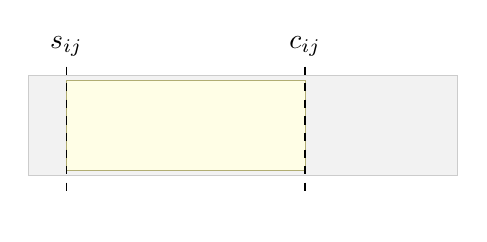
\begin{tikzpicture}
	\node[rectangle, draw=gray!40, fill=gray!10, minimum width=0.45\textwidth, minimum height=0.5in](bus) at (0,0){};	
	\node[rectangle, draw=yellow!50!black!70, fill=yellow!10, minimum width=0.25\textwidth, minimum height=0.45in](charge) at (-0.06\textwidth,0){};
	\node(topLeft) at (-0.185\textwidth,1){$s_{ij}$};
	\node(btmLeft) at (-0.185\textwidth,-1){};
	\draw[dashed, line width=0.5pt](topLeft) -- (btmLeft);
	\node(topRight) at (0.065\textwidth,1){$c_{ij}$};
	\node(btmRight) at (0.065\textwidth,-1){};
	\draw[dashed, line width=0.5pt](topRight) -- (btmRight);
\end{tikzpicture}
}%

	\subfloat[Discrete Charging Segments\label{fig:remainderB}]{
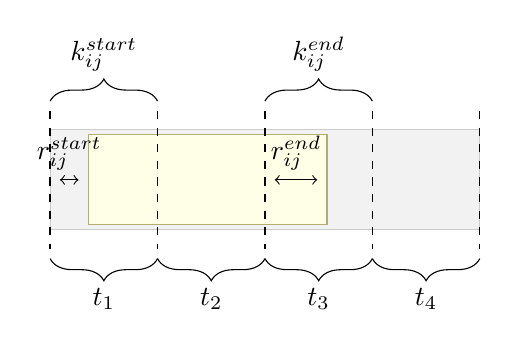
\begin{tikzpicture}
	\node[rectangle, draw=gray!40, fill=gray!10, minimum width=0.45\textwidth, minimum height=0.5in](bus) at (0,0){};	
	\node[rectangle, draw=yellow!50!black!70, fill=yellow!10, minimum width=0.25\textwidth, minimum height=0.45in](charge) at (-0.06\textwidth,0){};
	\node(top0) at (-0.225\textwidth,1){};
	\node(top1) at (-0.1125\textwidth,1){};
	\node(top2) at (0\textwidth,1){};
	\node(top3) at (0.1125\textwidth,1){};
	\node(top4) at (0.225\textwidth,1){};

	\node(btm0) at (-0.225\textwidth ,-1){};
	\node(btm1) at (-0.1125\textwidth,-1){};
	\node(btm2) at (0\textwidth      ,-1){};
	\node(btm3) at (0.1125\textwidth ,-1){};
	\node(btm4) at (0.225\textwidth  ,-1){}; 
	
	\draw[dashed, line width=0.5pt](top0) -- (btm0);
	\draw[dashed, line width=0.5pt](top1) -- (btm1);
	\draw[dashed, line width=0.5pt](top2) -- (btm2);
	\draw[dashed, line width=0.5pt](top3) -- (btm3);
	\draw[dashed, line width=0.5pt](top4) -- (btm4);

	\draw[decorate, decoration={brace, amplitude=8, mirror}](btm0.center) -- (btm1.center) node [midway, below=0.1in]{$t_1$};
	\draw[decorate, decoration={brace, amplitude=8, mirror}](btm1.center) -- (btm2.center) node [midway, below=0.1in]{$t_2$};
	\draw[decorate, decoration={brace, amplitude=8, mirror}](btm2.center) -- (btm3.center) node [midway, below=0.1in]{$t_3$};
	\draw[decorate, decoration={brace, amplitude=8, mirror}](btm3.center) -- (btm4.center) node [midway, below=0.1in]{$t_4$};

	\draw[decorate, decoration={brace, amplitude=8}](top0.center) -- (top1.center) node [midway, above=0.1in]{$k_{ij}^{\text{start}}$};
	\draw[decorate, decoration={brace, amplitude=8}](top2.center) -- (top3.center) node [midway, above=0.1in]{$k_{ij}^{\text{end}}$};


	\node(s0) at (-0.225\textwidth,0){};
	\node(s1) at (-0.185\textwidth,0){};
	\draw[<->](s0) -- node[above]{$r_{ij}^{\text{start}}$} ++ (s1); 
	
	\node(c0) at (0.065\textwidth,0){};
        \node(c1) at (0.0\textwidth,0){};
	\draw[<->](c0) -- node[above]{$r_{ij}^{\text{end}}$} ++ (c1); 
\end{tikzpicture} 
}
	\caption{Discretization of continuous charging intervals}
\end{figure}
